
%(BEGIN_QUESTION)
% Copyright 2008, Tony R. Kuphaldt, released under the Creative Commons Attribution License (v 1.0)
% This means you may do almost anything with this work of mine, so long as you give me proper credit

Suppose a control valve is used to throttle the flow of cooling water from a utility water header (constant pressure of 80 PSI) through the tube side of a shell-and-tube heat exchanger:

$$\includegraphics[width=15.5cm]{i03213x01.eps}$$

At full-open, the control valve needs to limit the cooling water flow rate to a maximum of 140 gallons per minute.  At that flow rate, the tubes inside the heat exchanger will drop 36 PSI of pressure across their length.  Calculate the $C_v$ rating for the control valve, and also estimate the nominal pipe size of the control valve (in inches).

\vskip 10pt

$C_v$ = \underbar{\hskip 50pt}

\vskip 10pt

Nominal pipe size = \underbar{\hskip 50pt}

\vskip 20pt \vbox{\hrule \hbox{\strut \vrule{} {\bf Suggestions for Socratic discussion} \vrule} \hrule}

\begin{itemize}
\item{} Explain how a shell-and-tube heat exchanger is constructed, and exactly how heat gets transferred from one fluid to another in such a device.
\item{} Identify the proper controller action, assuming a direct-acting temperature transmitter and a signal-to-close valve.
\item{} Identify some of the {\it loads} in this process control loop.  A ``load'' is some influencing factor on the process variable that is not directly regulated by the control loop.
\item{} What type of control valve and actuator are used in this application?
\end{itemize}

\underbar{file i03213}
%(END_QUESTION)





%(BEGIN_ANSWER)

\noindent
{\bf Partial answer:}

\vskip 10pt

$C_v$ = 21.1

%(END_ANSWER)





%(BEGIN_NOTES)

$$\Delta P = 80 - 36 = 44 \hbox{ PSID}$$

$$C_v = {Q \over \sqrt{\Delta P \over G_f}}$$

$$C_v = {140 \over \sqrt{44 \over 1}} = 21.11$$

\vskip 10pt

Assuming a $C_d$ value of 25 for a contoured ball valve:

$$d = \sqrt{C_v \over C_d}$$

$$d = \sqrt{21.11 \over 25} = 0.919$$

At a calculated pipe diameter of $d$ = 0.919, we are so close to 1 inch that this will likely be the proper size of control valve to use.

%INDEX% Final Control Elements, valve: sizing
%INDEX% Process: heat exchanger temperature/flow control (generic)

%(END_NOTES)


